\documentclass[a4paper]{scrreprt}

\usepackage[T1]{fontenc}
\usepackage[a4paper, total={6.5in, 9in}]{geometry}

% Imports:
\usepackage{bm}
\usepackage{tikz}
\usepackage{float}
\usepackage{minted}
\usepackage{amsmath}
\usepackage{amssymb}
\usepackage{booktabs}
\usepackage{palatino}
\usepackage{todonotes}
\usepackage{subcaption}

\usepackage[inline]{enumitem}
\setlist[description]{font=\normalfont}

\usepackage{nomencl}
\makenomenclature%


\definecolor{peach}{RGB}{247, 120, 107} % rgb(247, 120, 107)
\definecolor{rose}{RGB}{247,202,201} % rgb(247,202,201)
\definecolor{green}{RGB}{121, 199, 83} % rgb(121, 199, 83)
\definecolor{coffee}{RGB}{177,143,106} % rgb(177,143,106)
\definecolor{serenity}{RGB}{145,168,208} % rgb(145,168,208)
\definecolor{yellow}{RGB}{250,224,60} % rgb(250,224,60)
\definecolor{red}{RGB}{221,65,50} % rgb(221,65,50)
\definecolor{blue}{RGB}{3,79,132} % rgb(3,79,132)
\definecolor{limpet}{RGB}{152,221,222} % rgb(152,221,222)

\usetikzlibrary{shapes.geometric, arrows}
\tikzstyle{startstop} = [rectangle, rounded corners, minimum width=3cm, minimum height=1cm,text centered, draw=rose, fill=rose!80]
\tikzstyle{io} = [trapezium, trapezium left angle=70, trapezium right angle=110, minimum width=3cm, minimum height=1cm, text centered, draw=yellow, fill=yellow!80]
\tikzstyle{process} = [rectangle, minimum width=3cm, minimum height=1cm, text centered, draw=limpet, fill=limpet!80]
\tikzstyle{api} = [rectangle, minimum width=3cm, minimum height=1cm, text centered, draw=peach, fill=peach!80]
\tikzstyle{decision} = [diamond, minimum width=3cm, minimum height=1cm, text centered, draw=green, fill=green!80, text width=2.5cm]
\tikzstyle{arrow} = [thick,->,>=stealth, draw=coffee]

%% LABELS DEFINITIONS
\tikzstyle{orangeLabel} = [rectangle, rounded corners, text centered, draw=orange, fill=orange!80]
\tikzstyle{peachLabel} = [rectangle, rounded corners, text centered, draw=peach, fill=peach!80]
\tikzstyle{roseLabel} = [rectangle, rounded corners, text centered, draw=rose, fill=rose!80]
\tikzstyle{greenLabel} = [rectangle, rounded corners, text centered, draw=green, fill=green!80]
\tikzstyle{coffeeLabel} = [rectangle, rounded corners, text centered, draw=coffee, fill=coffee!80]
\tikzstyle{serenityLabel} = [rectangle, rounded corners, text centered, draw=serenity, fill=serenity!80]
\tikzstyle{yellowLabel} = [rectangle, rounded corners, text centered, draw=yellow, fill=yellow!80]
\tikzstyle{redLabel} = [rectangle, rounded corners, text centered, draw=red, fill=red!80]
\tikzstyle{blueLabel} = [rectangle, rounded corners, text centered, draw=blue, fill=blue!80]
\tikzstyle{limpetLabel} = [rectangle, rounded corners, text centered, draw=limpet, fill=limpet!80]


% Definitions:
\newcommand{\Lay}{\mathrm{l}}
\newcommand{\Back}{\mathrm{b}}

\newcommand{\Price}{P}

\newcommand\todoin[2][]{\todo[inline, caption={2do}, #1]{%
    \begin{minipage}{\textwidth-4pt}#2\end{minipage}}}

\newcommand\figwidth{0.9\textwidth}


\title{Cointegration Strategy}
\subtitle{Technical Report}

\author{Stratagem Technologies}


\begin{document}
\maketitle


\chapter{Background}
\section{Cointegration}
The basic intuition of the signal is that over a given look-back window there
may exist a (temporary) \emph{cointegrating} relationship between two time
series (e.g.\ price processes, scoring rates, etc\ldots) whose expected
stability may be exploited. Formally, the cointegration property means that
there exists a linear combination (portfolio) whose implied ``spread series''
is stationary and thus has a mean and variance that do not change with time
(time-homogeneous).


\section{Strategy}
\begin{figure}
    \centering
    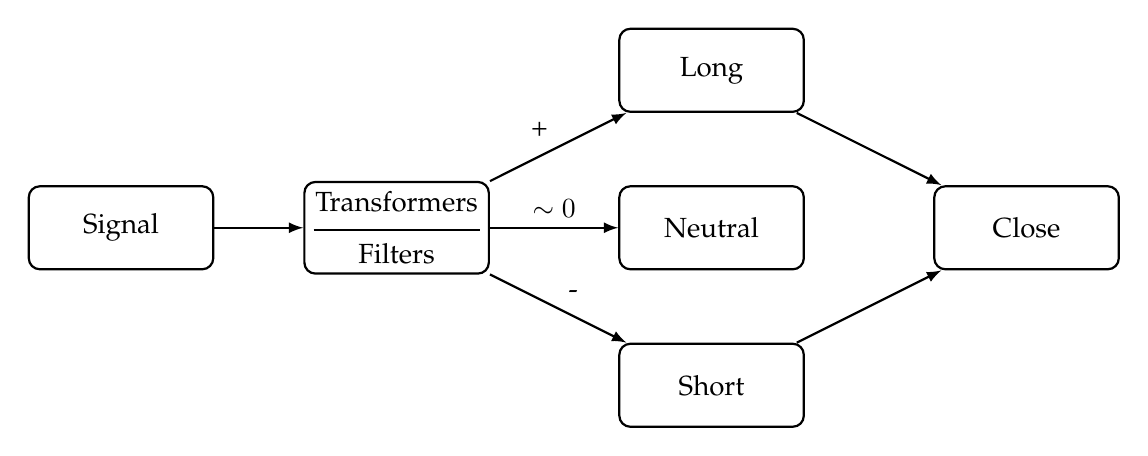
\begin{tikzpicture}[node distance=2cm, auto, thick]
        \tikzstyle{block} = [rectangle, draw, text width=6em, text centered,
        rounded corners, minimum height=3em]
        \tikzstyle{line} = [draw, -latex]

        \node [block] (node0) {Signal};
        \node [block, right of=node0, xshift=1.5cm] (node5)
            {Transformers\\[-0.5em]\noindent\rule{\linewidth}{0.6pt}\\Filters};

        \node [block, right of=node5, xshift=2cm] (node2) {Neutral};
        \node [block, above of=node2] (node1) {Long};
        \node [block, below of=node2] (node3) {Short};

        \node [block, right of=node2, xshift=2cm] (node4) {Close};

        \draw [line] (node0) -- (node5);

        \draw [line] (node5) --node {+} (node1);
        \draw [line] (node5) --node {$\sim 0$} (node2);
        \draw [line] (node5) --node {-} (node3);

        \draw [line] (node1) -- (node4);
        \draw [line] (node3) -- (node4);
    \end{tikzpicture}

    \caption{Structure of generic trading strategy which attempts to capture
    short-term trends in an asset's valuation.}\label{fig:strategy_basic}
\end{figure}

The fundamental building blocks of the strategy are very simple (see
Fig~\ref{fig:strategy_basic}):
\begin{enumerate}
    \item compute the cointegration signal;
    \item apply a sequence of filters and transformations to the signal;
    \item open a position based on the anticipated direction of the spread;
    \item close the position to lock in gains or losses.
\end{enumerate}

Each of the strategies considered herein --- for which the signals generation
processes are described in Chapter~\ref{ch:signals} --- have this structure.
The real complexity arises in the ``Signal'' and ``Transformers|Filters'' nodes
which contain our main decision making logic. For example, a typical strategy
might exploit the implied mean reversion in the spread by re-cast the spread
series into a vector of standard scores\footnote{Typically computed by
evaluating $\frac{x - \mu_x}{\sigma_x}$.} and using the current level of
deviation from the mean as an indication of the future direction; i.e.\ where a
large score would imply a negative trend due to reversion to the mean and
vice-versa.


\subsection{Interpreting signal values}
The signal, $\bm{\beta} \in \mathbb{R}$, takes the form of a real valued vector
of length $m$, where $m$ is the number of markets in the portfolio. The sign
and magnitude of each value dictates how to trade on each of the $m$ markets
(equivalently, stickers): negative values indicate short positions and, by
symmetry, positive values indicate long positions (see
Fig.~\ref{fig:signal2trade}). The absolute value is then used to assign
relative sizes to the trades in the portfolio; note that values close to zero
should likely be ignored since the resulting size is often negligible.

\begin{figure}
    \centering
    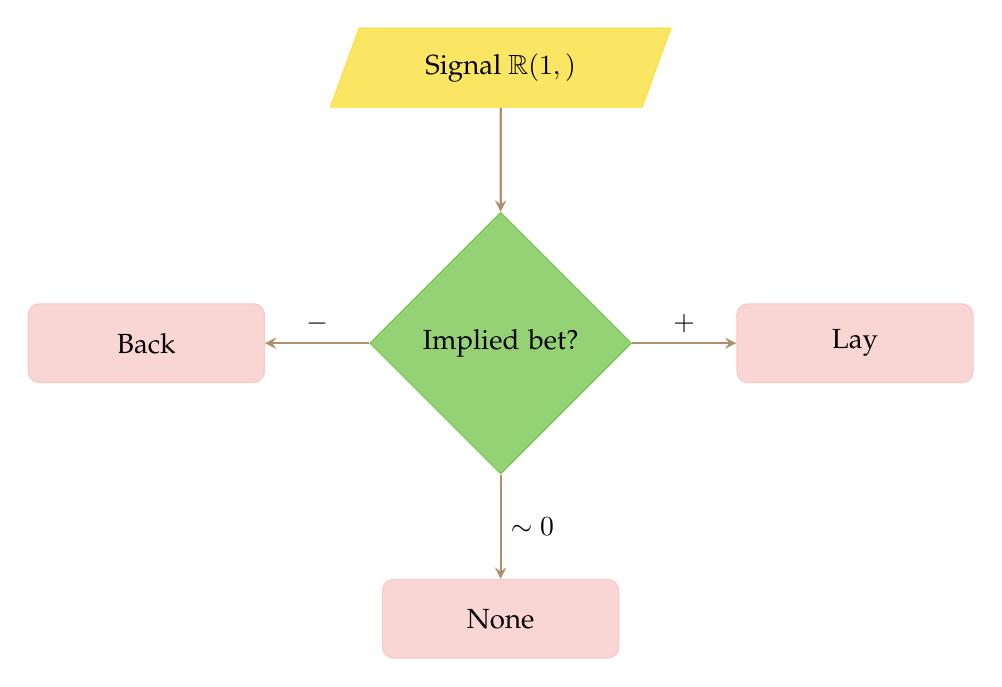
\begin{tikzpicture}[node distance=2cm]
        \node (node0) [io] {Signal $\mathbb{R}(1,)$};
        \node (node1) [decision, below of=node0, yshift=-1.5cm] {Implied bet?};

        \node (node2) [startstop, below of=node1, yshift=-1.5cm] {None};
        \node (node3) [startstop, left of=node1, xshift=-2.5cm] {Back};
        \node (node4) [startstop, right of=node1, xshift=2.5cm] {Lay};

        \draw [arrow] (node0) -- (node1);
        \draw [arrow] (node1) --node[anchor=west] {$\sim 0$} (node2);
        \draw [arrow] (node1) --node[anchor=south] {$-$} (node3);
        \draw [arrow] (node1) --node[anchor=south] {$+$} (node4);
    \end{tikzpicture}

    \caption{Illustration of generic signal to trade decision
    logic.}\label{fig:signal2trade}
\end{figure}


\subsection{Common strategy features}
\paragraph{Naming}
The cointegration strategy is written to support many underlying mechanisms for
generating a long/short signal based on an implied spread series. Further, it
arbitrarily supports any market pair for $m\geq2$. As such we need a clear
naming convention that indicates exactly \emph{what} we're trading on, and
\emph{what} method we're using to derive the signal. The following conventions
are imposed:
\begin{description}[leftmargin=!, labelwidth=8em]
    \item[\mintinline{python}{strategy_name}] For readability, it is suggested
        that the strategy name include ``coint''. For now the only concrete
        implementation of the strategy, based on market price processes, has
        the name: \textbf{coint\_mpc}.
    \item[\mintinline{python}{strategy_desc}] The strategy descriptor defines
        the method used inside the signal generator to extract a direction
        (prediction) from the spread series.
    \item[\mintinline{python}{strategy_code}] The strategy code should be used to add final details to the cointegration strategy such as which market to trade on.
    \item[\mintinline{python}{mnemonic}] This can be used to distinguish even
        further in case you wanted to do some specific tests, say with
        \mintinline{python}{MatchingMode.ALWAYS_MATCH}. Though the value of
        \mintinline{python}{mnemonic} does not affect anything in the code, it
        does allow for manual debugging and filtering in the database.
\end{description}


\paragraph{Parameters}
Though each iteration of the cointegration strategy may have it's own set of
parameters, some are common throughout:
\begin{description}[leftmargin=!, labelwidth=2em]
    \item[\mintinline{python}{LB}] the number of periods to include in the
        look-back window.
    \item[\mintinline{python}{SS}] the sub-sampling rate for the look-back
        window; i.e.\ for a value 2, we sample every other value\footnote{The
            sub-sampling rate is especially important when using
            computationally intensive methods for predicting changes in the
            spread series. For our purposes this will not be the case, though
        it is still informative to investigate it's impact on returns.}.
    \item[$\underbar{$t$}$] the minimum holding time for a given portfolio;
        for practical reasons this is lower bounded by the in-play delay.
    \item[$T$] the maximum holding time for a given portfolio; this is only
        comes into effect when no non-zero signal is observed.
    \item[$r_\text{TP}$] The take-profit threshold on expected portfolio
        returns.
    \item[$r_\text{SL}$] The stop-loss threshold on expected portfolio
        returns.
\end{description}


\begin{figure}
    \centering
    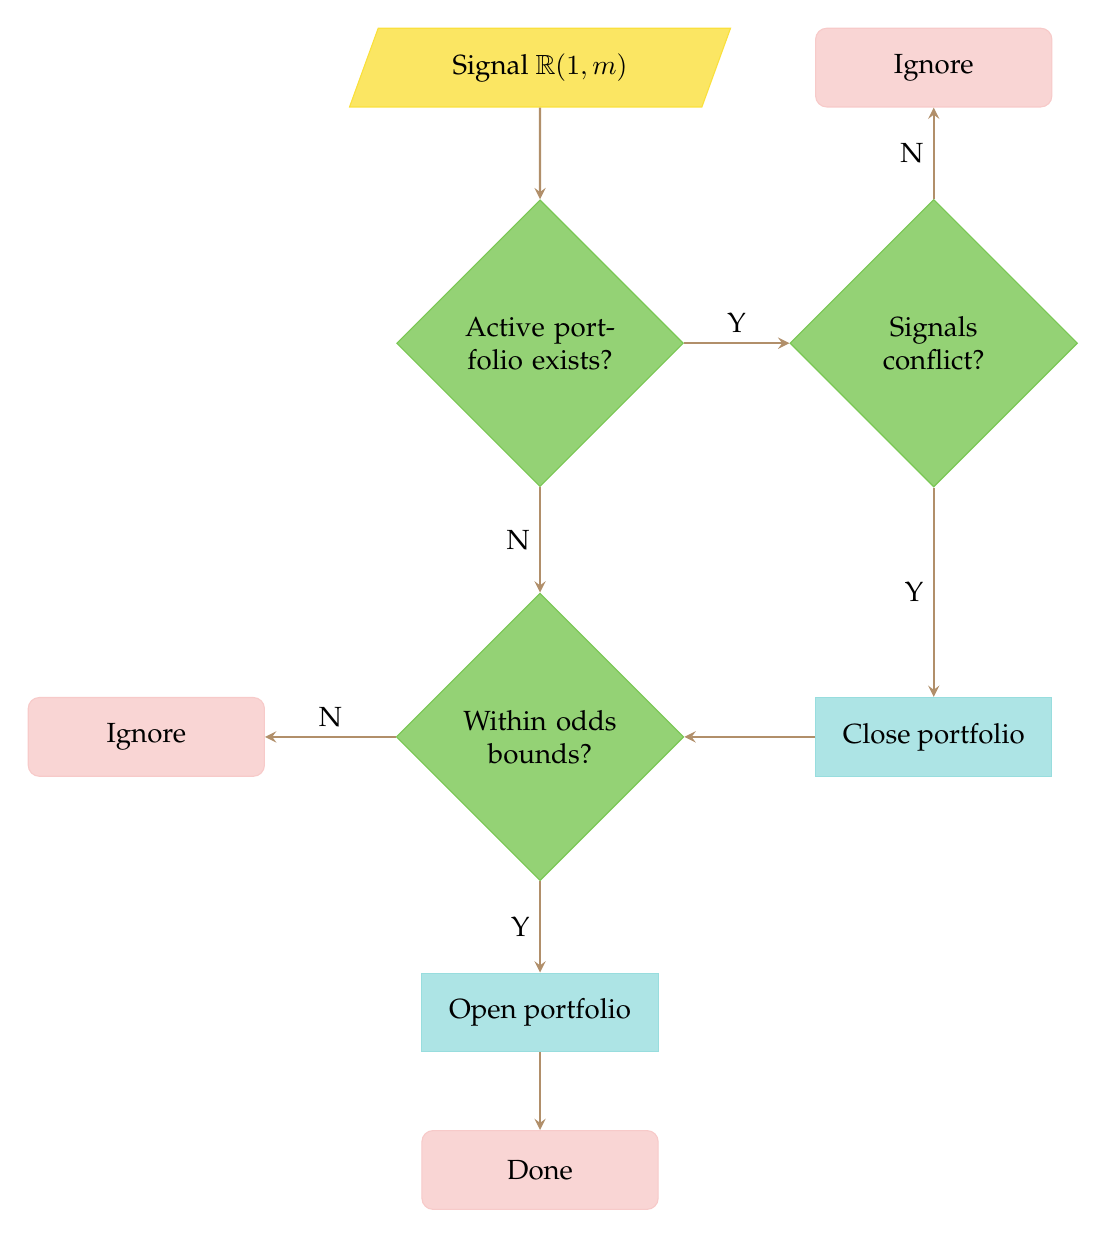
\begin{tikzpicture}[node distance=2cm]
        \node (node2) [io] {Signal $\mathbb{R}(1, m)$};
        \node (node3) [decision, below of=node2, yshift=-1.5cm] {Active portfolio exists?};

        \node (node11) [decision, below of=node3, yshift=-3cm] {Within odds bounds?};
        \node (node12) [startstop, left of=node11, xshift=-3cm] {Ignore};

        \node (node4) [decision, right of=node3, xshift=3cm] {Signals conflict?};
        \node (node8) [process, right of=node11, xshift=3cm] {Close portfolio};
        \node (node7) [startstop, above of=node4, yshift=1.5cm] {Ignore};

        \node (node9) [process, below of=node11, yshift=-1.5cm] {Open portfolio};
        \node (node10) [startstop, below of=node9] {Done};

        \draw [arrow] (node3) --node[anchor=south] {Y} (node4);
        \draw [arrow] (node4) --node[anchor=east] {N} (node7);

        \draw [arrow] (node3) --node[anchor=east] {N} (node11);
        \draw [arrow] (node2) -- (node3);
        \draw [arrow] (node8) -- (node11);
        \draw [arrow] (node4) --node[anchor=east] {Y} (node8);

        \draw [arrow] (node9) -- (node10);
        \draw [arrow] (node11) --node[anchor=south] {N} (node12);
        \draw [arrow] (node11) --node[anchor=east] {Y} (node9);
    \end{tikzpicture}

    \caption{\todo[inline]{Add description of this diagram and why it's common
    to all strategies.}}
\end{figure}

\begin{figure}
    \centering
    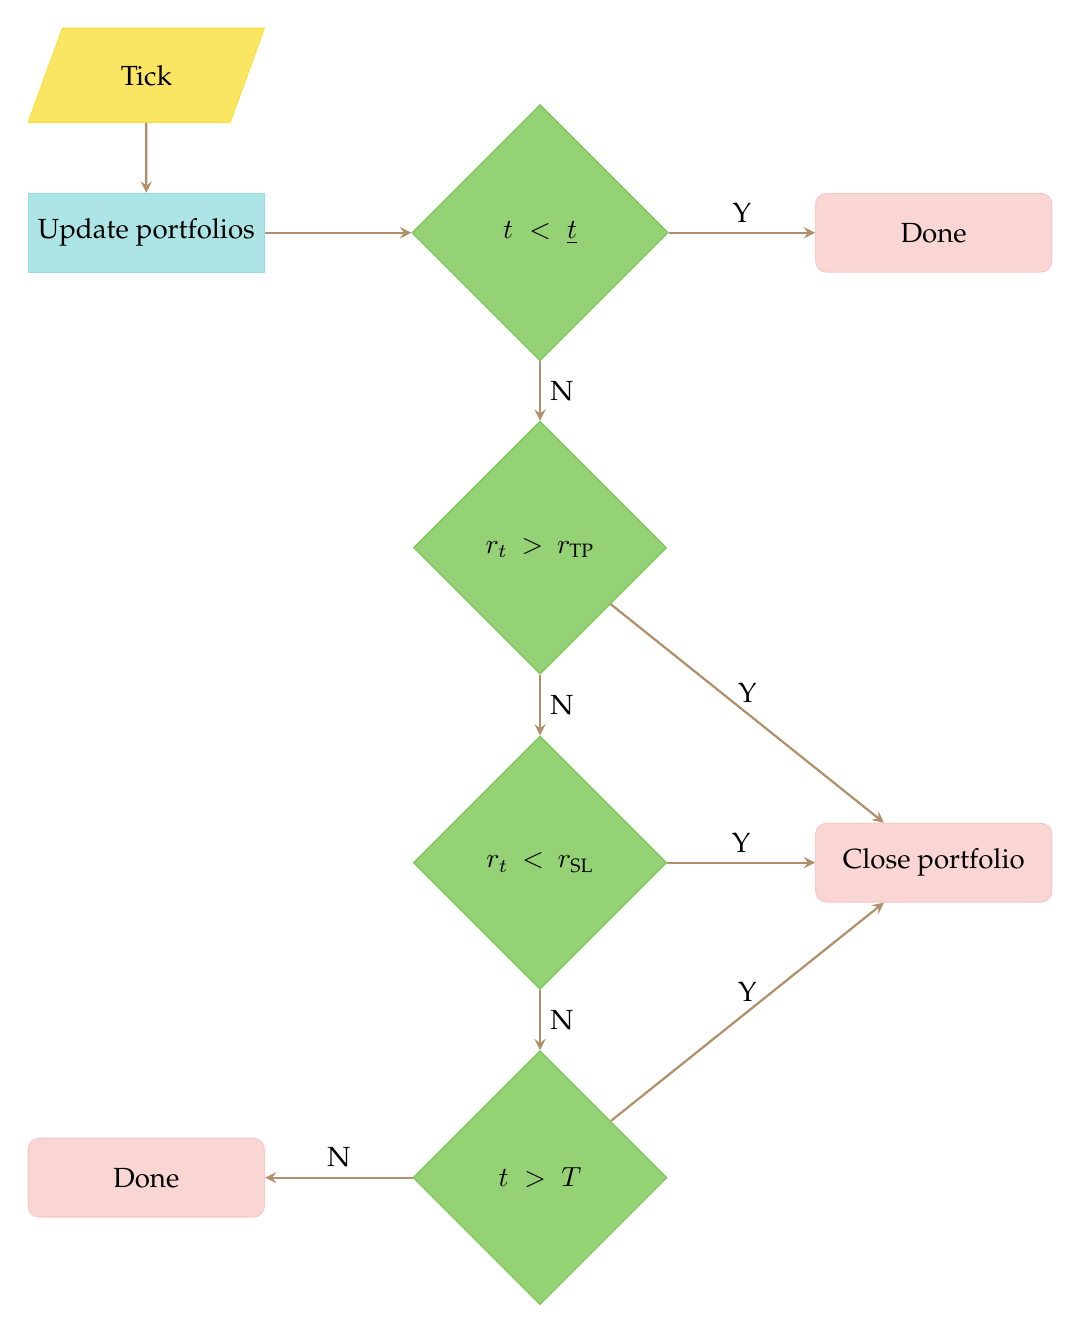
\begin{tikzpicture}[node distance=2cm]
        \node (node0) [io] {Tick};
        \node (node1) [process, below of=node0] {Update portfolios};

        \node (node2) [decision, right of=node1, xshift=3cm] {$t < \underbar{$t$}$};
        \node (node3) [decision, below of=node2, yshift=-2cm] {$r_t > r_\text{TP}$};
        \node (node4) [decision, below of=node3, yshift=-2cm] {$r_t < r_\text{SL}$};
        \node (node5) [decision, below of=node4, yshift=-2cm] {$t > T$};

        \node (node6) [startstop, right of=node2, xshift=3cm] {Done};
        \node (node7) [startstop, right of=node4, xshift=3cm] {Close portfolio};
        \node (node8) [startstop, left of=node5, xshift=-3cm] {Done};

        \draw [arrow] (node0) -- (node1);
        \draw [arrow] (node1) -- (node2);

        \draw [arrow] (node2) --node[anchor=south] {Y} (node6);
        \draw [arrow] (node3) --node[anchor=south] {Y} (node7);
        \draw [arrow] (node4) --node[anchor=south] {Y} (node7);
        \draw [arrow] (node5) --node[anchor=south] {Y} (node7);

        \draw [arrow] (node2) --node[anchor=west] {N} (node3);
        \draw [arrow] (node3) --node[anchor=west] {N} (node4);
        \draw [arrow] (node4) --node[anchor=west] {N} (node5);
        \draw [arrow] (node5) --node[anchor=south] {N} (node8);
    \end{tikzpicture}

    \caption{\todo[inline]{Add description of this diagram and why it's common
    to all strategies.}}
\end{figure}



\chapter{Basis Estimation}
A robust estimate of the basis vector is crucial for developing a trading
strategy with any confidence. While the Johansen procedure is very efficient
and produces good estimates in theory, the time series used in practice are
often very noisy and have periods of intermittent cointegration (structural
breaks) which can damage our overall estimate of the relationship. To improve
our estimate we use a system of ``weak'' experts and combine them to form
robust basis vector with, empirically speaking, much better convergence
properties.

The weak estimators are formed by applying the Johansen procedure over varying
data slices, such as a moving window for using the entire observed dataset up
to time $t$. One may then apply smoothing, such as (exponentially-weighted)
moving averages or Bayesian parameter estimation procedures, on top of this to
further improve robustness of each individual expert.

\section{Normal-Normal model}
We consider a univariate Gaussian model for the observed values of the basis
vector, $\mathcal{N}(\mu, \sigma^2)$, in which the variance is assumed known
but the mean is estimated. We let $D = (x_1, \ldots, x_n)$ be the data such
that the likelihood takes the form,
\begin{align}
    p(D \mid \mu, \sigma^2) &= \prod_{i=1}^n p(x_i \mid \mu, \sigma^2), \\
    &= (2\pi\sigma^2)^{-n/2}
           \exp\left[-\frac{1}{2\sigma^2} \sum_{i=1}^n (x_i - \mu)^2\right].
\end{align}
Assuming a constant $\sigma^2$, we have the following relationship,
\begin{align}
    p(D \mid \mu, \sigma^2) &\propto
        \exp\left[-\frac{n}{2\sigma^2}(\bar x - \mu)^2\right], \\
    &\propto \mathcal{N}(\bar x \mid \mu, \frac{\sigma^2}{n}).
\end{align}

For simplicity, we use the natural conjugate prior for $p(\mu) \propto
\mathcal{N}(\mu \mid \mu_0, \sigma_0^2)$ to obtain nice closed-form solutions
for the estimate updates. After some simple manipulation one obtains the following update rules:
\begin{align}
    \sigma_n^2 &= \frac{\sigma^2\sigma_0^2}{n\sigma_0^2 + \sigma^2}, \\
    \mu_n &= \sigma_n^2\left(\frac{\mu_0}{\sigma_0^2} + \frac{n\bar
        x}{\sigma^2}\right).
\end{align}

\subsection{Good priors}
It's important that a good prior, $p(\mu)$, is used in order to get an
practicable estimation of the basis early on. To do this, we look at the
historical distributions of basis vectors (Tab.~\ref{tab:bbprior}) and assume
that they are indicative of future relationships. For completeness, we include
the distributions for different periods of each match, where $\mu_0$ and
$\sigma_0$ are the mean and standard deviation on the prior, respectively.
\begin{table}
    \centering
    \begin{tabular}{@{\textbf}lllll@{}}
        \toprule
        & $\mu_0$ & $\sigma_0$ & $m$    & $c$    \\
        \midrule
        Whole match    & 0.4920  & 0.0634     & 0.0024 & 0.4986 \\
        \midrule
        First quarter  & 0.4954  & 0.1188     & 0.0033 & 0.5067 \\
        Second quarter & 0.4950  & 0.1138     & 0.0038 & 0.4893 \\
        Third quarter  & 0.4890  & 0.1132     & 0.0035 & 0.4865 \\
        Fourth quarter & 0.4915  & 0.1121     & 0.0016 & 0.5000 \\
        \midrule
        First half     & 0.4925  & 0.0938     & 0.0031 & 0.4959 \\
        Second half    & 0.4922  & 0.0834     & 0.0028 & 0.5025 \\
        \bottomrule
    \end{tabular}

    \caption{Emprirical prior distributions over the cointegration basis vector
    of basketball team scores between 06/2015 to 11/2017.}\label{tab:bbprior}
\end{table}

To further improve our estimate we can consider the relationship between the
natural handicap on the match and the means of the given basis distributions.
The gradient, $m$, and intercept, $c$, may then be used to form an adjusted
estimate of $\mu_0$, given by the following,
\begin{equation}
    \mu_0 \sim m\cdot\textrm{NH} + c,
\end{equation}
where $\textrm{NH}$ is the natural handicap.

\section{Combining estimators}
Based on Gareth's voting scheme technical report, we used a minimum variance
estimator (MVE) to combine the weak experts. This assumes that the individual
estimates are unbiased, which is likely untrue, but forms a decent first method
for combining in a single unbiased strong estimator. In practice one may know a
priori that some estimators should be weighted higher but we leave this is for
future work.

The MVE estimator produces the following weights for a system of $K$
estimators,
\begin{equation}
    w_i = \frac{1/\sigma_i^2}{\sum_{k=1}^K(1/\sigma_k^2)},
\end{equation}
which yields a weighted average for the mean, with variance given by,
\begin{equation}
    \sigma^2 = \left(\sum_{k=1}^K \frac{1}{\sigma_k^2} \right)^{-1}.
\end{equation}


\section{Case Study}
To illustrate the effectiveness of the MVE estimator, we present an
example\footnote{Note that the results do carry across matches, this is not
just a one off.} using a basketball match between the Dallas Mavericks and the
New York Knicks.

\begin{figure}[H]
    \centering
    \includegraphics[width=\figwidth]{img/estimation/scores.png}

    \caption{Scores of teams A (red) and B (blue) for the basketball match with
    event id 2352975.}\label{fig:estimation:scores}
\end{figure}

\begin{figure}[H]
    \begin{subfigure}[b]{0.49\textwidth}
        \centering
        \includegraphics[width=\figwidth]{img/estimation/windowed_raw.png}

        \caption{Raw}
    \end{subfigure}
    \hfill
    \begin{subfigure}[b]{0.49\textwidth}
        \centering
        \includegraphics[width=\figwidth]{img/estimation/windowed_bayes.png}

        \caption{Bayes}
    \end{subfigure}

    \caption{Estimations of the cointegration basis (first component) given
    using a moving window.}\label{fig:estimation:windowed}
\end{figure}

\begin{figure}[H]
    \begin{subfigure}[b]{1.0\textwidth}
        \centering
        \includegraphics[width=\figwidth]{img/estimation/cumulative_raw.png}

        \caption{Raw}
    \end{subfigure}
    \\[1em]
    \begin{subfigure}[b]{0.49\textwidth}
        \centering
        \includegraphics[width=\figwidth]{img/estimation/cumulative_bayes.png}

        \caption{Bayes}
    \end{subfigure}
    \hfill
    \begin{subfigure}[b]{0.49\textwidth}
        \centering
        \includegraphics[width=\figwidth]{img/estimation/cumulative_ewma.png}

        \caption{Exponentially-weighted moving average}
    \end{subfigure}

    \caption{Estimations of the cointegration basis (first component) given
    using an accumulated window of all observed
    estimations.}\label{fig:estimation:cumulative}
\end{figure}

\begin{figure}[H]
    \centering
    \includegraphics[width=\figwidth]{img/estimation/mve.png}

    \caption{Minimum variance estimation of the cointegration basis using a
    combination of Bayesian windowed estimators and exponentially-weighted
    moving average cumulative estimators.}\label{fig:estimation:mve}
\end{figure}

\begin{figure}[H]
    \centering
    \includegraphics[width=\figwidth]{img/estimation/mse.png}

    \caption{Distribution of the mean squared error of the estimation against
    the best estimate across all recorded matches in the period 06/2015 to
    11/2017. The mean (red line) is quoted along with the $3\sigma$ confidence
    interval.}\label{fig:estimation:mse}
\end{figure}



\chapter{Strategies}\label{ch:signals}
\section{Common}
Thus far, the strategies have been constrained to multi-sport variants, none
have been specific to a single sport; though the next step would be to exploit
any causal relationship between the cointegration spread of basketball team
scores and market prices. These are all located in the
\mintinline{python}{stratagem-systematic} repository. Some of the common
utilities that you should probably make use are also in the
\mintinline{python}{stratagem-research-base} repo. The main ones to use and extend are:
\begin{enumerate}
    \item \mintinline{python}{OnlineCointegrationModelProvider} --- This
        utility (see sgmsystematic/trading/providers/model) takes tick data as
        input (not necessarily prices) and return the basis vectors for each of
        the stickers in the group. It makes use of the static methods in the
        \mintinline{python}{CointegrationTradingSignalService} class ( see
        sgmresearchbase/analysis/cointegration).
    \item \mintinline{python}{MPCSignalGenerator} --- This is the main
        component used to generate trading signals for the MPC trading
        strategy. It makes use of subclasses of the
        \mintinline{python}{CointegrationTradingSignalService} class and
        converts tick data into bases and finally into a directional trading
        signal to be used by the trader.
    \item \mintinline{python}{Portfolio} --- This class keeps track of a
        position opened on multiple markets and computes the expected return
        given any partial/full executions and the current market prices. It
        also has some utility plotting methods which are especially useful for
        debugging and evaluating performance online.
\end{enumerate}

I've included as many useful utilties for generating signals, tracking ticks
and smoothing estimations, etc, in the research base repo. All are fully
documented and tested. I would advise going over the MPC strategy first and
getting an idea about the pipeline to convert tick data into an actual trading
strategy. The next task will likely want to be to incorporate the improved
estimator (for which there are many possible parameterisations) and to build
and investigate a strategy deriving from the team scores and exploiting causul
relationships with the market.

\subsection{Notes from discussions with Gareth}
Some of the main points are:
\begin{enumerate}
    \item Improve the mean reversion signal by using robustified Bollinger
        bands and/or control charts rather than a simple estimation of the
        mean.
    \item Investigate the best ways to sample the team scores and thus the
        market prices.
    \item Investigate causality between scores and prices using Granger
        causality and/or an explicit model of the lead-lag relationship.
\end{enumerate}

\section{MPC}
The main strategy developed was the market price cointegration (MPC) strategy.

\subsection*{Parameters}
The strategy descriptor tells the framework which pair to trade and provides
arguments to that type.  For example, one pair that has been implemented is
\mintinline{python}{FT12_TGOU}, which corresponds to the full-time moneyline
and total games over/under markets. We may also choose to provide parameters to
this pair, the exact specification of which are dictated by the implementation.
Consider, for example, trading FT12, A versus B, on exclusively ATP matches.
Such a code would take the following form: \textbf{ft12\_tennis.ATP}. Note that
the pair and it's arguments come before and after the period, respectively.
Some further examples are given below:
\begin{itemize}
    \item \textbf{ft12\_tennis.ATP} --- full-time moneyline, A versus B, on ATP
        matches.
    \item \textbf{ft12\_tgou.ATP} --- full-time moneyline versus total games
        over/under, on ATP matches.
\end{itemize}


\subsection{Mark 0 (COR)}
\begin{figure}
    \centering
    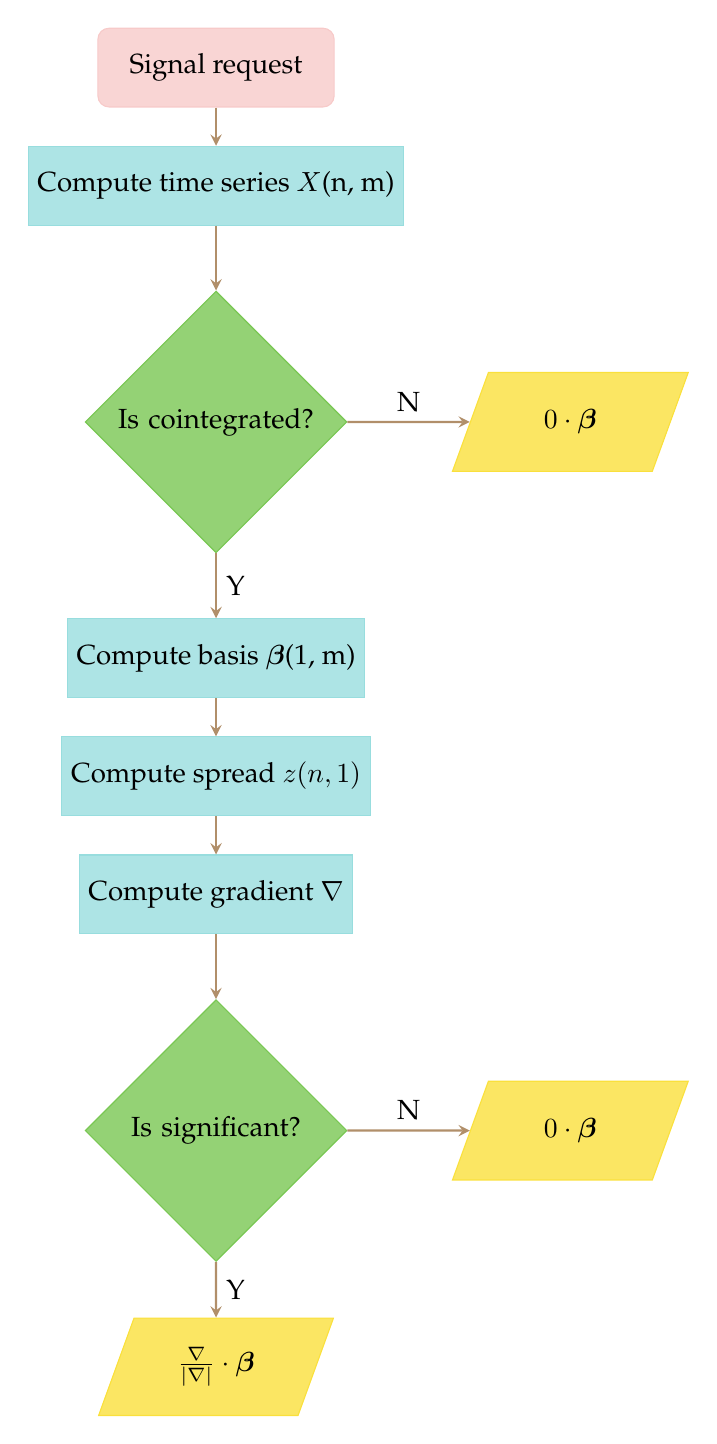
\begin{tikzpicture}[node distance=1.5cm]
        \node (node0) [startstop] {Signal request};
        \node (node1) [process, below of=node0] {Compute time series $X$(n, m)};

        \node (node2) [decision, below of=node1, yshift=-1.5cm] {Is cointegrated?};
        \node (node3) [io, right of=node2, xshift=3cm] {$0\cdot \bm{\beta}$};

        \node (node4) [process, below of=node2, yshift=-1.5cm] {Compute basis $\bm{\beta}$(1, m)};
        \node (node5) [process, below of=node4] {Compute spread $z(n, 1)$};
        \node (node6) [process, below of=node5] {Compute gradient $\nabla$};

        \node (node7) [decision, below of=node6, yshift=-1.5cm] {Is significant?};
        \node (node8) [io, below of=node7, yshift=-1.5cm] {$\frac{\nabla}{|\nabla|} \cdot \bm{\beta}$};
        \node (node9) [io, right of=node7, xshift=3cm] {$0\cdot \bm{\beta}$};

        \draw [arrow] (node0) -- (node1);
        \draw [arrow] (node1) -- (node2);
        \draw [arrow] (node2) --node[anchor=south] {N} (node3);
        \draw [arrow] (node2) --node[anchor=west] {Y} (node4);
        \draw [arrow] (node4) -- (node5);
        \draw [arrow] (node5) -- (node6);
        \draw [arrow] (node6) -- (node7);
        \draw [arrow] (node7) --node[anchor=south] {N} (node9);
        \draw [arrow] (node7) --node[anchor=west] {Y} (node8);
    \end{tikzpicture}
\end{figure}


\subsection{Mark 1 (MR)}
\begin{figure}
    \centering
    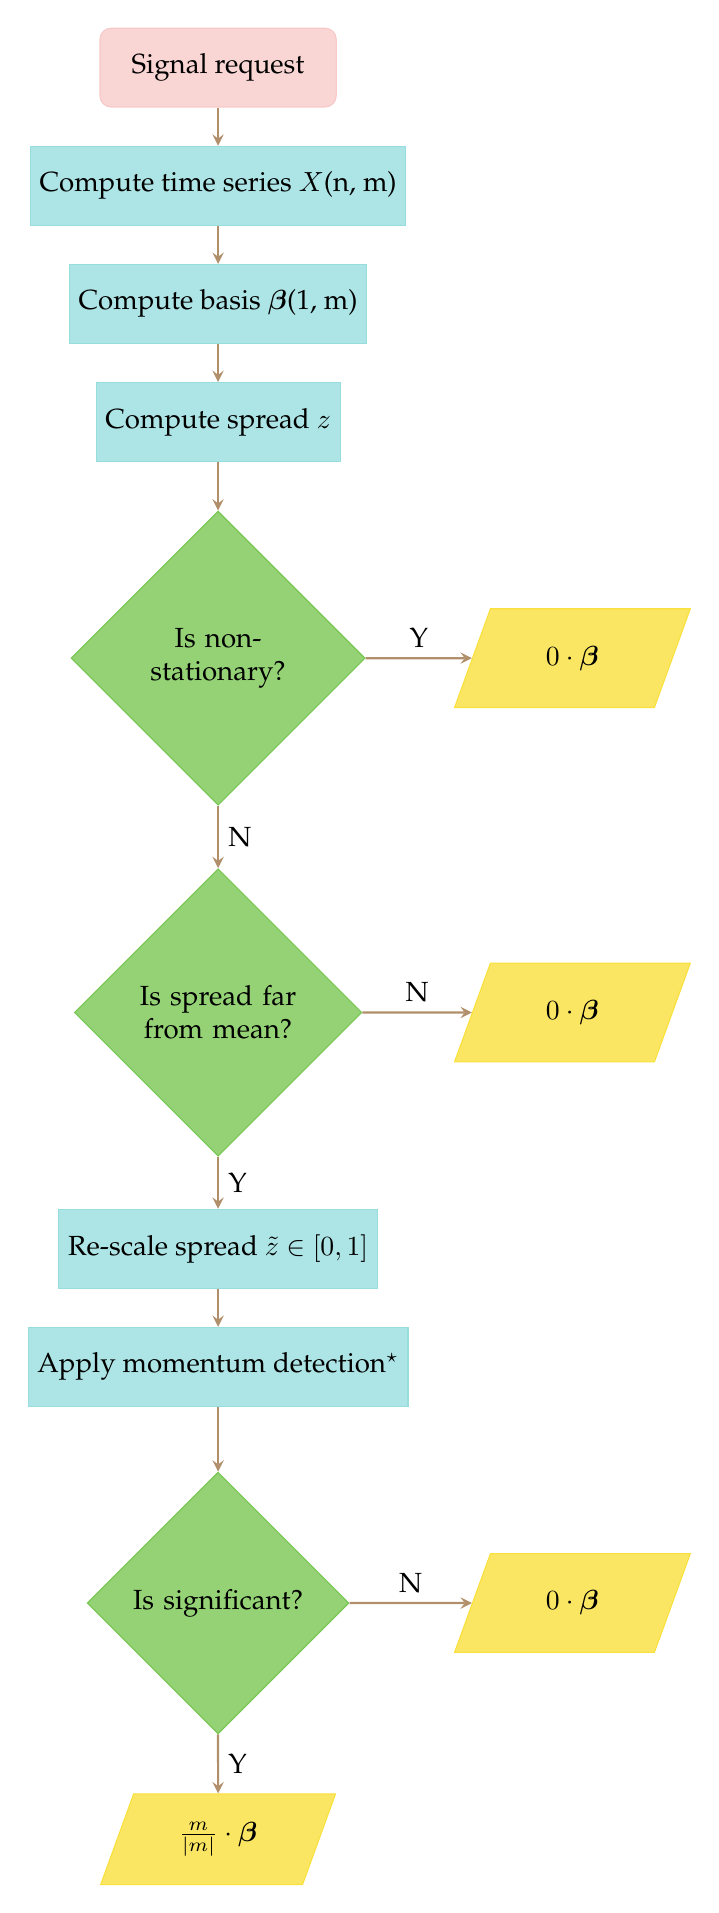
\begin{tikzpicture}[node distance=1.5cm]
        \node (node0) [startstop] {Signal request};
        \node (node1) [process, below of=node0] {Compute time series $X$(n, m)};
        \node (node2) [process, below of=node1] {Compute basis $\bm{\beta}$(1, m)};
        \node (node3) [process, below of=node2] {Compute spread $z$};
        \node (node4) [decision, below of=node3, yshift=-1.5cm] {Is non-stationary?};
        \node (node5) [decision, below of=node4, yshift=-3cm] {Is spread far from mean?};
        \node (node6) [process, below of=node5, yshift=-1.5cm] {Re-scale spread $\tilde z \in [0, 1]$};
        \node (node7) [process, below of=node6] {Apply momentum detection$^\star$};
        \node (node8) [decision, below of=node7, yshift=-1.5cm] {Is significant?};
        \node (node9) [io, below of=node8, yshift=-1.5cm] {$\frac{m}{|m|} \cdot \bm{\beta}$};

        \node (node10) [io, right of=node4, xshift=3cm] {$0\cdot \bm{\beta}$};
        \node (node11) [io, right of=node5, xshift=3cm] {$0\cdot \bm{\beta}$};
        \node (node12) [io, right of=node8, xshift=3cm] {$0\cdot \bm{\beta}$};

        \draw [arrow] (node0) -- (node1);
        \draw [arrow] (node1) -- (node2);
        \draw [arrow] (node2) -- (node3);
        \draw [arrow] (node3) -- (node4);
        \draw [arrow] (node4) --node[anchor=west] {N} (node5);
        \draw [arrow] (node5) --node[anchor=west] {Y} (node6);
        \draw [arrow] (node6) -- (node7);
        \draw [arrow] (node7) -- (node8);
        \draw [arrow] (node8) --node[anchor=west] {Y} (node9);

        \draw [arrow] (node4) --node[anchor=south] {Y} (node10);
        \draw [arrow] (node5) --node[anchor=south] {N} (node11);
        \draw [arrow] (node8) --node[anchor=south] {N} (node12);
    \end{tikzpicture}
\end{figure}


\subsection{Mark 2 (Hybrid)}



\appendix
\chapter{Appendix}
\section{Preliminary Evaluation}
For simplicity, we begin with an evaluation of the signal over A/B outright
winner market pairs for tennis ATP matches between 2017/08/01 and 2017/09/30
(amounts to a total of 347 events where 220 are actually traded). Though the
existence of cointegration within this pairing is unclear, there is a much
stronger guarantee of liquidity which makes for less sparse backtest results.

The following assumptions are made about the environment
\begin{enumerate}
    \item Zero in-play delay.
    \item Immediate execution at either the mid-price or top of the book ---
        this also implies that we do not consider prevalent effects such as
        adverse selection.
    \item Perfect connection such that we experience zero latency and no loss of
        messages in transit to the exchange.
    \item We do not consider path dependency (perhaps due to randomness) or any
        of the complexities associated with cashing out, amounting to an
        assumption of infinite liquidity.
\end{enumerate}

\subsection{Mid-price execution}
Here we assume that the agent is executed favourably at the mid-prices of the
two legs. Thus, the strategy effectively tracks the spread series, taking a
long, short or neutral position based on the cointegration signal.

A few key observations:
\begin{enumerate}
    \item For the short holding period we consider here (until the next time
        step) short lookback windows are favourable
        (Fig.~\ref{fig:mp_nodelay:pnl}).
    \item The sub-sampling rate appears to have a considerable effect on the
        performance, though this relationship is not the same of all lookback
        windows. Crucially, for the 200 period window, larger values for the
        sampling-rate (sampling less) have lower associated variance.
    \item The proportion of wins to losses behaves in the opposite way, where
        larger values of the sub-sampling rate have increased variance and a
        greater proportion of outlier cases (Fig.~\ref{fig:mp_nodelay:propwl}).
    \item The consistency ratio appears to be best for larger lookback windows
        and low sampling rates.
\end{enumerate}

\begin{figure}[H]
    \centering
    \includegraphics[width=\figwidth]{img/mp_nodelay.png}

    \caption{}\label{fig:mp_nodelay:pnl}
\end{figure}

\begin{figure}[H]
    \centering
    \includegraphics[width=\figwidth]{img/mp_nodelay_propwl.png}

    \caption{}\label{fig:mp_nodelay:propwl}
\end{figure}

\begin{figure}[H]
    \centering
    \includegraphics[width=\figwidth]{img/mp_nodelay_cr.png}

    \caption{}\label{fig:mp_nodelay:cr}
\end{figure}

\subsection{Spread crossing execution}
Here we assume that the agent always crosses the spread, walking the book in
each of the two legs.

A few observations:
\begin{enumerate}
    \item The strategy performs very poorly when crossing the spread on every
        trade opportunity. This is likely due to the fact that the holding time
        is very short, so the cost of entry/exit are applied very frequently.
    \item Win/loss proportion is also very poor. Further the consistency ratio
        shows that the strategy was never profitable on a step-by-step basis.
        Again, we need longer and/or more informed holding times.
\end{enumerate}

\begin{figure}[H]
    \centering
    \includegraphics[width=\figwidth]{img/sp_nodelay.png}

    \caption{}\label{fig:sp_nodelay:pnl}
\end{figure}

\begin{figure}[H]
    \centering
    \includegraphics[width=\figwidth]{img/sp_nodelay_propwl.png}

    \caption{}\label{fig:sp_nodelay:propwl}
\end{figure}

\begin{figure}[H]
    \centering
    \includegraphics[width=\figwidth]{img/sp_nodelay_cr.png}

    \caption{}\label{fig:sp_nodelay:cr}
\end{figure}


\end{document}
